\newpage
\maketitle
\begin{center}
\Large \textbf{第6章 统计套利策略} \quad 
\end{center}
\begin{abstract}
在本章中,我们将利用卡尔曼滤波技术,设计统计套利策略,利用我们的量化交易研究平台进行回测,初步验证策略的正确性。
并将GARCH模型用于实际金融时间序列数据拟合。
\end{abstract}
\section{统计套利策略}
统计套利策略是一种市场中性策略,在实际中有大量应用。
\subsection{数据获取}
我们要研究交易策略,首先要获取历史交易数据,在本节中,我们将讲述如何通过baostock的接口,来获取历史交易数据。我们之所以选择baostock接口,因为baostock可以提供免费的6分钏的日内交易数据,这在免费数据中是很少见的。不过我们这一篇中,我们只研究日线交易数据。baostock接口网站:
\lstset{language=BASH}
\begin{lstlisting}
http://baostock.com/baostock/index.php
\end{lstlisting}
获取股票历史交易记录非常简单,甚至都不用注册用户,例如我们想获取工商银行2006到至2018年数据,根据baostock的规定,工商银行的股票代码为601398.sh,程序如下所示:
\lstset{language=PYTHON, caption={baostock获取股票历史行情数据}, label={c000015}}
\begin{lstlisting}
import baostock as bs
import pandas as pd

class BsCnaDaily(object):
    def __init__(self):
        self.name = 'BsADaily'
        
    def get_history_data(self, stock_code, start_date, end_date):
        '''
        获取A股日线行情历史数据
        @param stock_code 股票代码,如工商银行为:sh.601398
        @param start_date 开始日期,格式yyyy-MM-dd
        @param end_date 结束日期,格式yyyy-MM-dd
        @return 获取成功返回True,否则返回False
        @version v0.0.1 闫涛 2019-04-22
        '''
        lg = bs.login()
        if lg.error_code != '0':
            print('login respond  error_msg:'+lg.error_msg)
            return False, lg.error_msg
        rs = bs.query_history_k_data_plus(stock_code,
                "date,code,open,high,low,close,preclose,volume,amount,adjustflag,turn,tradestatus,pctChg,isST",
                start_date=start_date, end_date=end_date,
                frequency="d", adjustflag="3")
        if rs.error_code != '0':
            print('query_history_k_data_plus respond  error_msg:'+rs.error_msg)
            return False,rs.error_msg
        data_list = []
        while (rs.error_code == '0') & rs.next():
            data_list.append(rs.get_row_data())
        result = pd.DataFrame(data_list, columns=rs.fields)
        result.to_csv('./data/{0}.csv'.format(stock_code), index=False)
        bs.logout()
        return True
\end{lstlisting}
调用方法如下所示:
\lstset{language=PYTHON, caption={baostock获取股票历史行情数据示例}, label={c000016}}
\begin{lstlisting}
import csv
import pandas as pd
import matplotlib.pyplot as plt
from core.quotation.bs_cna_daily import BsCnaDaily

class TpsaDataset(object):
    def __init__(self):
        self.name = 'TpsaDataset'
        
    @staticmethod
    def get_quotation_data(stocks):
        '''
        获取交易对行情数据
        @params stocks np.array [0][...]和[1][...]分别代表交易对
            对于交易对:[0]{stock_code, start_date, end_date, eft_name}
            其中eft_name也是数据文件保存的名字,stocks共有两条记录,由
            调用者负责保证
        '''
        print(stocks[0]['stock_code'])
        bs_cna_daily = BsCnaDaily()
        # 工商银行(股票代码60开头的是上海)
        bs_cna_daily.get_history_data(stocks[0]['stock_code'], 
                    stocks[0]['start_date'], stocks[0]['end_date'], 
                    stocks[0]['etf_name'])
        bs_cna_daily.get_history_data(stocks[1]['stock_code'], 
                    stocks[1]['start_date'], stocks[1]['end_date'], 
                    stocks[1]['etf_name'])
            
    @staticmethod
    def draw_close_price_curve(stock_files):
        '''
        绘制股票收益率曲线
        @stock_files 交易对股票行情文件名,共有两个
        '''
        print('绘制收盘价曲线...')
        etf0_prices = TpsaDataset.read_close_prices(stock_files[0])
        etf1_prices = TpsaDataset.read_close_prices(stock_files[1])
        plt.title('close price curve')
        plt.plot(etf0_prices)
        plt.plot(etf1_prices)
        plt.show()
    
    @staticmethod
    def read_close_prices(stock_file):
        '''
        读取股票收盘价数据时间序列
        @param stock_file 股票行情文件
        @return 股票收盘价的list
        '''
        close_prices = []
        with open(stock_file, 'r', newline='') as fd:
            rows = csv.reader(fd)
            header = next(rows)
            print('header:{0}'.format(header))
            for row in rows:
                close_prices.append(float(row[4]))
        return close_prices
        
    @staticmethod
    def read_close_price_pd(stock_file):
        dateparse = lambda x: pd.datetime.strptime(x, '%Y-%m-%d')
        prices = pd.read_csv(stock_file, encoding='utf-8', 
                parse_dates=['Date'], date_parser=dateparse, 
                index_col='Date')
        print(prices.values[:, 3])
\end{lstlisting}
\subsection{卡尔曼滤波策略}
在本例中,我们将工商银行收盘价作为自变量,将建设银行收盘价作为因变量。按照卡尔曼滤波框架,我们将建设银行的收盘价视为可观测状态$y_{t}$,而建设银行收盘价与工商银行收盘价之比,包括斜率和截距,视为系统验证状态,将工商银行收盘价视为观测矩阵,这样就组成了一个卡尔滤波模型。系统在刚开始运行时,我们拿一部分历史数据运行卡尔曼滤波器,通过EM算法,估计出卡尔曼滤波器中的参数,之后再根据历史数据运行回测流程。\newline
我们首先运行kalman.filter方法,求出系统的状态,然后根据工商银行收盘价和filter方法返回的系统状态中的斜率和截距,求出建设银行的计算值,将建设银行计算值与建设银行收盘价真实值相减得天误差,然后将其与观察向量计算中的误差的标准差相比较,如果小于负的标准差,则买入建设银行股票,并按斜率比例卖出对应数量的工商银行股份;如果大于标准差,则卖出建设银行股票,并按斜率比例买入对应数量的工商银行股票。具体代码如下所示:
\lstset{language=PYTHON, caption={卡尔曼滤波协整模型交易对策略}, label={c000017}}
\begin{lstlisting}
from __future__ import print_function

from math import floor
import math

import numpy as np

from qstrader.price_parser import PriceParser
from qstrader.event import (SignalEvent, EventType)
from qstrader.strategy.base import AbstractStrategy
from pykalman import KalmanFilter


class TpsaStrategy(AbstractStrategy):
    """
    Requires:
    tickers - The list of ticker symbols
    events_queue - A handle to the system events queue
    """
    def __init__(
        self, tickers, events_queue, equity, ts0, ts1
    ):
        self.tickers = tickers
        self.events_queue = events_queue
        self.equity = equity
        self.time = None
        self.latest_prices = np.array([-1.0, -1.0])
        self.invested = None

        self.delta = 1e-4
        self.wt = self.delta / (1 - self.delta) * np.eye(2)
        self.vt = 1e-3
        self.theta = np.zeros(2)
        self.P = np.zeros((2, 2))
        self.R = None

        self.days = 0
        self.qty = 20000
        self.cur_hedge_qty = self.qty
        
        self.yt_state = 0
        self.buy_price = 0.0
        
        self.ts0 = ts0
        self.ts1 = ts1
        self.kalman_mode = 1
        
        xt_means, xt_covs = self.train_kalman_filter(ts0, ts1)
        slope = xt_means[-1][0]
        # 将80%资金按1:slope比例购买ts1和ts0
        price0 = ts0[-1]
        price1 = ts1[-1]
        print('type:{0}; shape:{1}'.format(type(price0), ts0[-1].shape))
        amount = self.equity * 0.1
        amount1 = amount / (1 + slope)
        amount0 = amount * (slope / (1+slope))
        self.qty1 = int(math.floor(amount1 / price1))
        self.qty1_0 = self.qty1
        self.qty0 = int(math.floor(amount0 / price0))
        self.qty0_0 = self.qty0
        amt1 = self.qty1 * price1
        amt0 = self.qty0 * price0
        self.equity -= (amt0 + amt1)
        self.equity_0 = self.equity
        self.events_queue.put(SignalEvent(self.tickers[0], "BOT", self.qty0))
        print('购买{0}:数量:{1};价格:{2}'.format(self.tickers[0], self.qty0, self.ts0[-1]))
        self.events_queue.put(SignalEvent(self.tickers[1], "BOT", self.qty1))
        print('购买{0}:数量:{1};价格:{2}'.format(self.tickers[1], self.qty1, self.ts1[-1]))
        print('现金:{0}'.format(self.equity))
        
        self.ts0 = np.array([])
        self.ts1 = np.array([])
        self.deltas = np.array([])
        
        

    def _set_correct_time_and_price(self, event):
        """
        Sets the correct price and event time for prices
        that arrive out of order in the events queue.
        """
        # Set the first instance of time
        if self.time is None:
            self.time = event.time
        
        # Set the correct latest prices depending upon 
        # order of arrival of market bar event
        price = event.adj_close_price/float(
            PriceParser.PRICE_MULTIPLIER
        )
        if event.time == self.time:
            if event.ticker == self.tickers[0]:
                self.latest_prices[0] = price
            else:
                self.latest_prices[1] = price
        else:
            self.time = event.time
            self.days += 1
            self.latest_prices = np.array([-1.0, -1.0])
            if event.ticker == self.tickers[0]:
                self.latest_prices[0] = price
            else:
                self.latest_prices[1] = price

    def train_kalman_filter(self, ts0, ts1, mode=1):
        """
        Utilise the Kalman Filter from the PyKalman package
        to calculate the slope and intercept of the regressed
        ETF prices.
        """
        delta = 1e-5
        mu0 = np.zeros(2)
        sigma0 = np.ones((2, 2))
        Q = delta / (1 - delta) * np.eye(2)
        At = np.eye(2)
        Ct = np.vstack(
            [ts0, np.ones(ts0.shape)]
        ).T[:, np.newaxis]
        R = 1.0
        self.kf = KalmanFilter(
            n_dim_obs=1,
            n_dim_state=2,
            initial_state_mean=mu0,
            initial_state_covariance=sigma0,
            transition_matrices=At,
            observation_matrices=Ct,
            observation_covariance=R,
            transition_covariance=Q
        )
        yt = ts1
        #state_means, state_covs = kf.em(observations).filter(observations)
        if mode != 1:
            xt_means, xt_covs = self.kf.filter(yt)
        else:
            xt_means, xt_covs = self.kf.em(yt).filter(yt)
        return xt_means, xt_covs


    def calculate_signals(self, event):
        mode = 2
        if event.type == EventType.BAR:
            self._set_correct_time_and_price(event)
            # Only trade if we have both observations
            if all(self.latest_prices > -1.0):
                # kalman.filter_update
                self.ts0 = np.append(self.ts0, self.latest_prices[0])
                self.ts1 = np.append(self.ts1, self.latest_prices[1])
                if self.days < 100:
                    return
                if self.days % 30 == 0:
                    mode = 1
                xt_means, x_convs = self.train_kalman_filter(self.ts0, self.ts1, mode=2)
                slope = xt_means[-1][0]
                intercept = xt_means[-1][1]
                yt_hat = self.ts0[-1] * slope + intercept
                delta = yt_hat - self.ts1[-1]
                self.deltas = np.append(self.deltas, delta)
                threshold = np.std(self.deltas)
                if delta < -threshold:
                    # 卖掉0买入1
                    qty0 = int(math.floor(self.qty * slope))
                    self.events_queue.put(SignalEvent(self.tickers[0], "SLD", qty0))
                    self.qty0 -= qty0
                    self.equity += qty0 * self.latest_prices[0]
                    self.events_queue.put(SignalEvent(self.tickers[1], "BOT", self.qty))
                    self.qty1 += self.qty
                    self.equity -= self.qty * self.latest_prices[1]
                    print('    买入{0}:数量:{1};价格:{2};金额:{3}'.format(
                            self.tickers[1], self.qty, self.latest_prices[1], 
                            self.qty*self.latest_prices[1])
                    )
                    print('     卖出{0}:数量:{1};价格:{2};金额:{3}'.format(
                            self.tickers[0], qty0, self.latest_prices[0],
                            qty0*self.latest_prices[0]
                    ))
                    total = self.equity + self.qty0 * self.latest_prices[0] + self.qty1 * self.latest_prices[1]
                    print('########### 总资产:{0}={1}+{2}+{2}'.format(total, self.equity, 
                            self.qty0 * self.latest_prices[0], self.qty1 * self.latest_prices[1]))
                elif delta > threshold:
                    # 买入0卖出1
                    self.events_queue.put(SignalEvent(self.tickers[1], "SLD", self.qty))
                    self.qty1 -= self.qty
                    self.equity += self.qty * self.latest_prices[1]
                    qty0 = int(math.floor(self.qty * slope))
                    self.events_queue.put(SignalEvent(self.tickers[0], "BOT", qty0))
                    self.qty0 += qty0
                    self.equity -= qty0 * self.latest_prices[0]
                    print('    买入{0}:数量:{1};价格:{2};金额:{3}'.format(
                            self.tickers[0], qty0, self.latest_prices[0], 
                            self.qty*self.latest_prices[0])
                    )
                    print('     卖出{0}:数量:{1};价格:{2};金额:{3}'.format(
                            self.tickers[1], self.qty, self.latest_prices[1],
                            qty0*self.latest_prices[1]
                    ))
                    total = self.equity + self.qty0 * self.latest_prices[0] + self.qty1 * self.latest_prices[1]
                    print('########### 总资产:{0}={1}+{2}+{2}'.format(total, self.equity, 
                            self.qty0 * self.latest_prices[0], self.qty1 * self.latest_prices[1]))
\end{lstlisting}
另外,在程序中需要注意的部分为我们每隔一定的交易日,会重新使用EM算法来估计卡尔曼滤波器的参数,这样可以使我们的估计更加准确。
\subsection{卡尔曼滤波引擎}
我们在策略引擎中,初始化策略,调用平台进行回测,统计回测效果,代码如下所示:
\lstset{language=PYTHON, caption={卡尔曼滤波策略引擎}, label={c000018}}
\begin{lstlisting}
import calendar
import datetime
import numpy as np
from qstrader import settings
from qstrader.strategy.base import AbstractStrategy
from qstrader.position_sizer.naive import NaivePositionSizer
from qstrader.event import SignalEvent, EventType
from qstrader.compat import queue
from qstrader.trading_session import TradingSession
from qstrader.price_handler.bscna_daily_csv_bar import BscnaDailyCsvBarPriceHandler

import matplotlib.pyplot as plt
from app.tpsa.tpsa_dataset import TpsaDataset



from app.tpsa.tpsa_strategy import TpsaStrategy

class TpsaEngine(object):
    def __init__(self):
        self.name = 'QhEngine'
        
    def startup(self):
        testing = False
        config = settings.load_config()
        tickers = ['ICBC', 'CBC']
        # 读取用于估计卡尔曼滤波参数的时间序列
        ts0 = np.array(TpsaDataset.read_close_prices('./data/{0}_train.csv'.format(tickers[0])))
        ts1 = np.array(TpsaDataset.read_close_prices('./data/{0}_train.csv'.format(tickers[1])))
        
        self.title = [
            '基于卡尔曼滤波器的交易对策略'
        ]
        self.initial_equity = 1000000.0
        self.start_date = datetime.datetime(2017, 1, 1)
        self.end_date = datetime.datetime(2019, 4, 23)
        # Use the Monthly Liquidate And Rebalance strategy
        self.events_queue = queue.Queue()
        self.strategy = TpsaStrategy(
            tickers, self.events_queue, self.initial_equity, ts0, ts1
        )
        self.run(config, testing, tickers) 

    def run(self, config, testing, tickers):
        # Use the Naive Position Sizer where
        # suggested quantities are followed
        position_sizer = NaivePositionSizer()
        # Set up the backtest
        backtest = TradingSession(
            config, self.strategy, tickers,
            self.initial_equity, self.start_date, self.end_date,
            self.events_queue, title=self.title,
            position_sizer=position_sizer,
            price_handler=BscnaDailyCsvBarPriceHandler(
                config.CSV_DATA_DIR, self.events_queue,
                tickers, start_date=self.start_date,
                end_date=self.end_date
            )
        )
        results = backtest.start_trading(testing=testing)
        print('最后金额:{0}'.format(self.strategy.equity))
        
        total = self.strategy.equity + self.strategy.qty0 * \
                self.strategy.latest_prices[0] + \
                self.strategy.qty1 * self.strategy.latest_prices[1]
        print('########### 总资产:{0}={1}+{2}+{3}'.format(
                total, self.strategy.equity, 
                self.strategy.qty0 * self.strategy.latest_prices[0], 
                self.strategy.qty1 * self.strategy.latest_prices[1]
        ))
        delta0 = self.strategy.qty0 - self.strategy.qty0_0
        amt0 = 0.0
        if delta0 > 0:
            amt0 = self.strategy.latest_prices[0] * delta0
        else:
            amt0 = -self.strategy.latest_prices[0] * delta0
        delta1 = self.strategy.qty1 - self.strategy.qty1_0
        amt1 = 0.0
        if delta1 > 0:
            amt1 = self.strategy.latest_prices[1] * delta1
        else:
            amt1 = -self.strategy.latest_prices[1] * delta1
            
        print('initial:{0} vs final {1}'.format(self.strategy.equity_0, self.strategy.equity+amt0+amt1))
        
        return results
        
    
    def prepare_data(self):
        stocks = [
            {
                'stock_code': 'sh.601398',
                'start_date': '2019-03-01',
                'end_date': '2019-04-29',
                'etf_name': 'ICBC'
            }, 
            {
                'stock_code': 'sh.601939',
                'start_date': '2019-03-01',
                'end_date': '2019-04-29',
                'etf_name': 'CBC'
            }
        ]
        TpsaDataset.get_quotation_data(stocks)
        stock_files = [
            './data/{0}.csv'.format(stocks[0]['etf_name']),
            './data/{0}.csv'.format(stocks[1]['etf_name'])
        ]
        TpsaDataset.draw_close_price_curve(stock_files)

\end{lstlisting}
\subsection{运行结果}
通过如下代码可以运行这个策略的回测:
\lstset{language=PYTHON, caption={运行卡尔曼滤波策略引擎}, label={c000019}}
\begin{lstlisting}
        tpsaEngine = TpsaEngine()
        tpsaEngine.startup()
\end{lstlisting}
运行程序后,得到累积收益率曲线如下所示:
\begin{figure}[H]
	\caption{累积收益率曲线}
	\label{f000058}
	\centering
	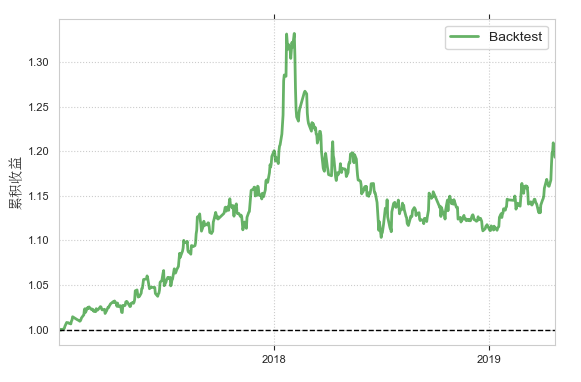
\includegraphics[height=10cm]{images/f000058}
\end{figure}
在图形中有一段收益率非常高,但是在那个时间段,由于我们采用的是统计套利策略,并不会处理暴涨暴跌的情况,因此这段行情并没有把握住。关于这一点我们将在下一节进行讨论。\newline
年化夏普比曲线:
\begin{figure}[H]
	\caption{年化夏普比曲线}
	\label{f000059}
	\centering
	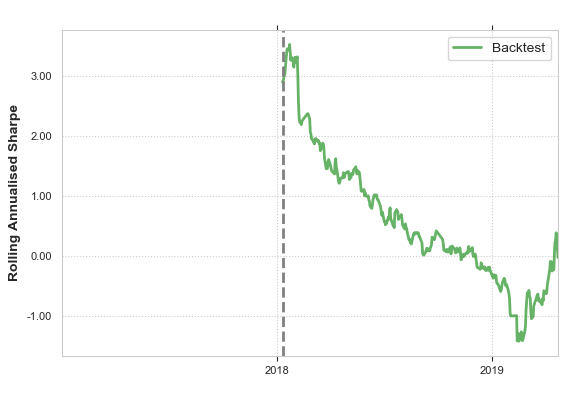
\includegraphics[height=10cm]{images/f000059}
\end{figure}
策略最大回撤图如下所示:
\begin{figure}[H]
	\caption{策略最大回撤}
	\label{f000060}
	\centering
	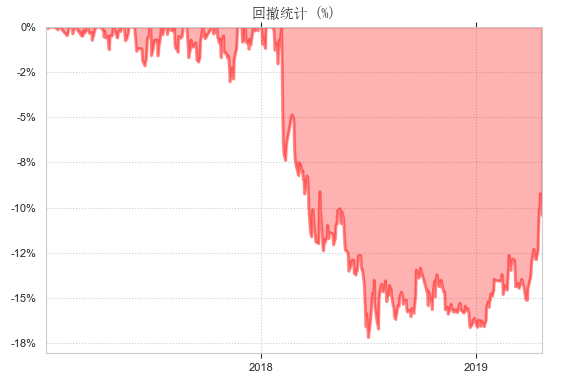
\includegraphics[height=10cm]{images/f000060}
\end{figure}
由于我们没在最高点时抛出股票,因此最大回撤图形上显得有些差,但是最后效果上面来看,应该还能说得过去。\newline
月收益率曲线:
\begin{figure}[H]
	\caption{月收益率曲线}
	\label{f000061}
	\centering
	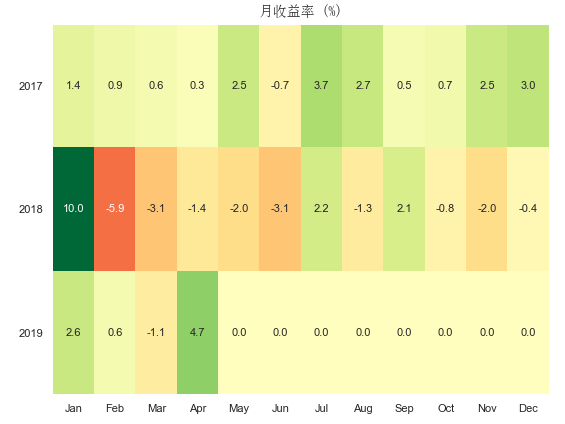
\includegraphics[height=10cm]{images/f000061}
\end{figure}
年化收益率:
\begin{figure}[H]
	\caption{年化收益率曲线}
	\label{f000062}
	\centering
	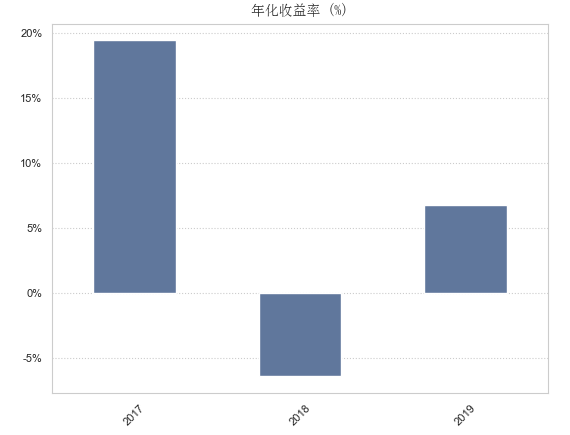
\includegraphics[height=10cm]{images/f000062}
\end{figure}
总体统计信息:
\begin{figure}[H]
	\caption{总体统计信息}
	\label{f000063}
	\centering
	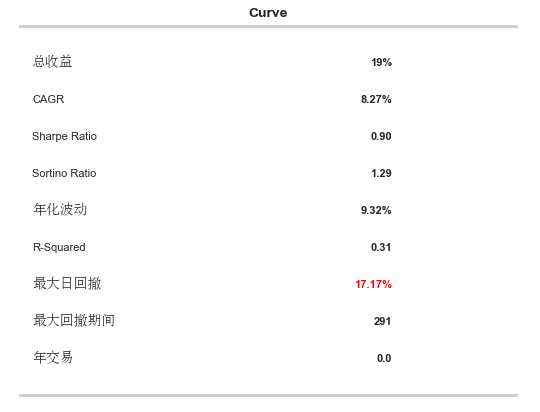
\includegraphics[height=10cm]{images/f000063}
\end{figure}
由上图可以看出,夏普比为0.88,通常较好的交易策略夏比应该在1以上,所以本策略还不是一个特别好的策略。
策略最终结果如下所示:
\begin{figure}[H]
	\caption{最终结果}
	\label{f000064}
	\centering
	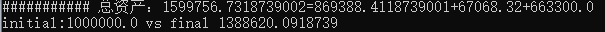
\includegraphics[height=1cm]{images/f000064}
\end{figure}
在这个策略中,我们假设我们会长期持有50000股工商银行和50000股建设银行,每次波动对冲时交易20000股,初始时我们流动资金是100万,不采用资金杠杆,在回测结束时,我们将工商银行和建设银行恢复回各50000股,然后计算流动资金。由结果可以看出,我们在持股情况未变化的情况下,流动资金变为138.86万,实现了38.86万的盈利。这证明我们的策略还是基本可行的。策略最终夏普比为0.9,也处于较为理想的数值区间。
\subsection{讨论}
虽然我们基于卡尔曼滤波的协整模型,实际表现还算中规中矩,是一个可接受的交易策略,但是毕竟我们希望得到更高的收益率,在这一节中我们就来分析一下,为什么我们的交易策略收益率不是特别高呢?\newline
首先,我们没有采用资金杠杆,因为我们知道,交易对之间的相对波动较小,交易所还会收取交易费和印花税等费用,因此即使判断正确,每一单的盈利也是非常小的。如果我们可以使用资金杠杆,通常统计套利策略资金杠杆可以达到3$\sim$5倍,这样我们的收益率就会提高到100\%以上(扣除杠杆利息),这就是一个相当不错的交易策略了。例如,LTCM专门做德国国债和意大利国债交易对的基金,其资金杠杆高达数万倍。当然,使用资金杠杆,在放大收益率的同时,也会放大风险,如果判断失误,损失将非常惨重。事实上,红极一时的LTCM基金,就是因为一个决策失误,导致资金链断裂,最终破产的。\newline
其次,基于协整模型的交易对策略,虽然是一种市场中性策略,但是在市场剧烈波动时,由于信号具有非平稳性,在此期间应该停止交易,这通常通过交易平台的风控模块来实现,但是我们这个策略中没有风控模块。下图是工商银行和建设银行收盘价走势曲线图:
\begin{figure}[H]
	\caption{工商银行(蓝)和建设银行(红)收盘价曲线}
	\label{f000065}
	\centering
	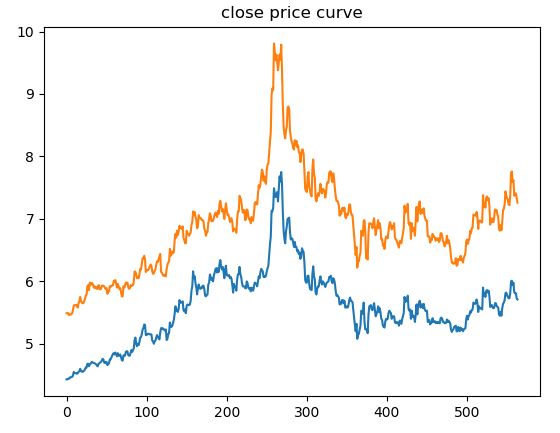
\includegraphics[height=5cm]{images/f000065}
\end{figure}
由图\ref{f000065}可以看出,二者收盘价走势非常具有一致性,因此作为协整模型的交易对是没有问题的。但是大家请注意,在我们进行回测中间,二者的股价都有一次暴涨和回调,在这种行情下,显然应该采取以跟踪短期趋势为主的程序化交易CPA策略,而本章中的策略,基本没有对这一过程进行特别处理,这显然是需要优化的。